%!TEX program = xelatex
%!TEX root = geometria_analitica.tex
%%Usar makeindex -s indexstyle.ist arquivo.idx no terminal para gerar o {\'\i}ndice remissivo agrupado por inicial
%%Ap\'os executar pdflatex arquivo

\chapter{Qu\'adricas} % (fold)
\label{cha:quadricas}

Em $\real^3$ estamos interessados em objetos definidos por uma equa\c{c}\~ao de segundo grau em $x$, $y$ e $z$ da forma
\begin{equation}\label{equacao_quadrica}
	ax^2 + by^2 + cz^2 + dxy + exz + fyz + gx + hy + iz + j = 0.
\end{equation}

O conjunto de pontos em $\real^3$ satisfazendo uma equa\c{c}\~ao da forma \eqref{equacao_quadrica} \'e chamado de uma \textbf{qu\'adrica}. Observe que pelo menos um dos n\'umeros $a$, $b$, $c$, $d$, $e$ ou $f$ deve ser n\~ao nulo.\index{Qu\'adricas}

Nosso principal objetivo ser\'a tentar simplificar a equa\c{c}\~ao \eqref{equacao_quadrica} de modo que seja poss{\'\i}vel identificar que objeto tal equa\c{c}\~ao representa.


\section{Esfera} % (fold)
\label{sec:esfera}
\begin{definicao}
	Uma \textbf{esfera} \'e uma qu\'adrica com equa\c{c}\~ao na forma\index{Qu\'adricas!Esfera}
	\begin{equation}\label{equacao_esfera}
		x^2 + y^2 + z^2 = r^2.
	\end{equation}
\end{definicao}

\begin{figure}[h]
	\centering
	\caption{Esfera: $x^2 + y^2 + z^2 = r^2$}
	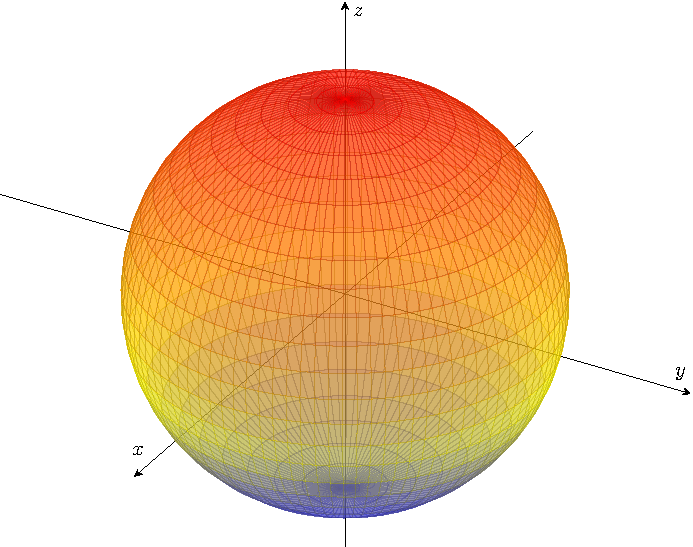
\includegraphics[scale=0.7]{esfera.pdf}
\end{figure}

\section{Elips\'oide} % (fold)
\label{sec:elipsoide}
\begin{definicao}
	Um \textbf{elips\'oide} \'e uma qu\'adrica descrita pela equa\c{c}\~ao
	\begin{equation}\label{equacao_elipsoide}
		\dfrac{x^2}{a^2} + \dfrac{y^2}{b^2} + \dfrac{z^2}{c^2} = 1
	\end{equation}
	onde os n\'umeros reais $a$, $b$ e $c$ s\~ao positivos e pelo menos dois deles s\~ao distintos.\index{Qu\'adricas!Elips\'oide}
\end{definicao}

Considere o plano $\pi: z = k$. Qual a interse\c{c}\~ao de $\pi$ com o elips\'oide de equa\c{c}\~ao \eqref{equacao_elipsoide}? A interse\c{c}\~ao \'e dada pelo sistema
\[
	\begin{cases}
		\dfrac{x^2}{a^2} + \dfrac{y^2}{b^2} + \dfrac{z^2}{c^2} = 1\\
		z = k,
	\end{cases}
\]
isto \'e, pela equa\c{c}\~ao
\begin{equation}\label{intersecao_elipsoide_planoz}
	\dfrac{x^2}{a^2} + \dfrac{y^2}{b^2} = 1 - \dfrac{k^2}{c^2}.
\end{equation}

Se $k^2 > c^2$, ent\~ao a equa\c{c}\~ao \eqref{intersecao_elipsoide_planoz} n\~ao admite solu\c{c}\~ao pois $1 - k^2/c^2 < 0$. Assim seja $k^2 \le c^2$, isto \'e, $-c \le k \le c$. Se $k = c$, ent\~ao a interse\c{c}\~ao \'e o ponto $(0,0,c)$ e se $k = -c$ \'e o ponto $(0,0,-c)$. Ent\~ao seja $-c < k < c$ e denote $p = 1 - k^2/c^2$. Podemos reescrever \eqref{intersecao_elipsoide_planoz} como
\begin{equation}\label{resultado_intersecao_elipsoide_planoz}
	\dfrac{x^2}{pa^2} + \dfrac{y^2}{pb^2} = 1.
\end{equation}

Se $a = b$, ent\~ao a equa\c{c}\~ao \eqref{resultado_intersecao_elipsoide_planoz} \'e uma circunfer\^encia. Se $a \ne b$, ent\~ao a equa\c{c}\~ao \eqref{resultado_intersecao_elipsoide_planoz} descreve uma elipse.

De modo an\'alogo, se tomarmos $\pi : x = k$ ou $\pi : y = k$, as interse\c{c}\~oes ser\~ao sempre ou conjunto vazio ou um ponto ou uma circunfer\^encia ou uma elipse.
\begin{figure}[h]
	\centering
	\caption{Elips\'oide: $\dfrac{x^2}{a^2} + \dfrac{y^2}{b^2} + \dfrac{z^2}{c^2} = 1$}
	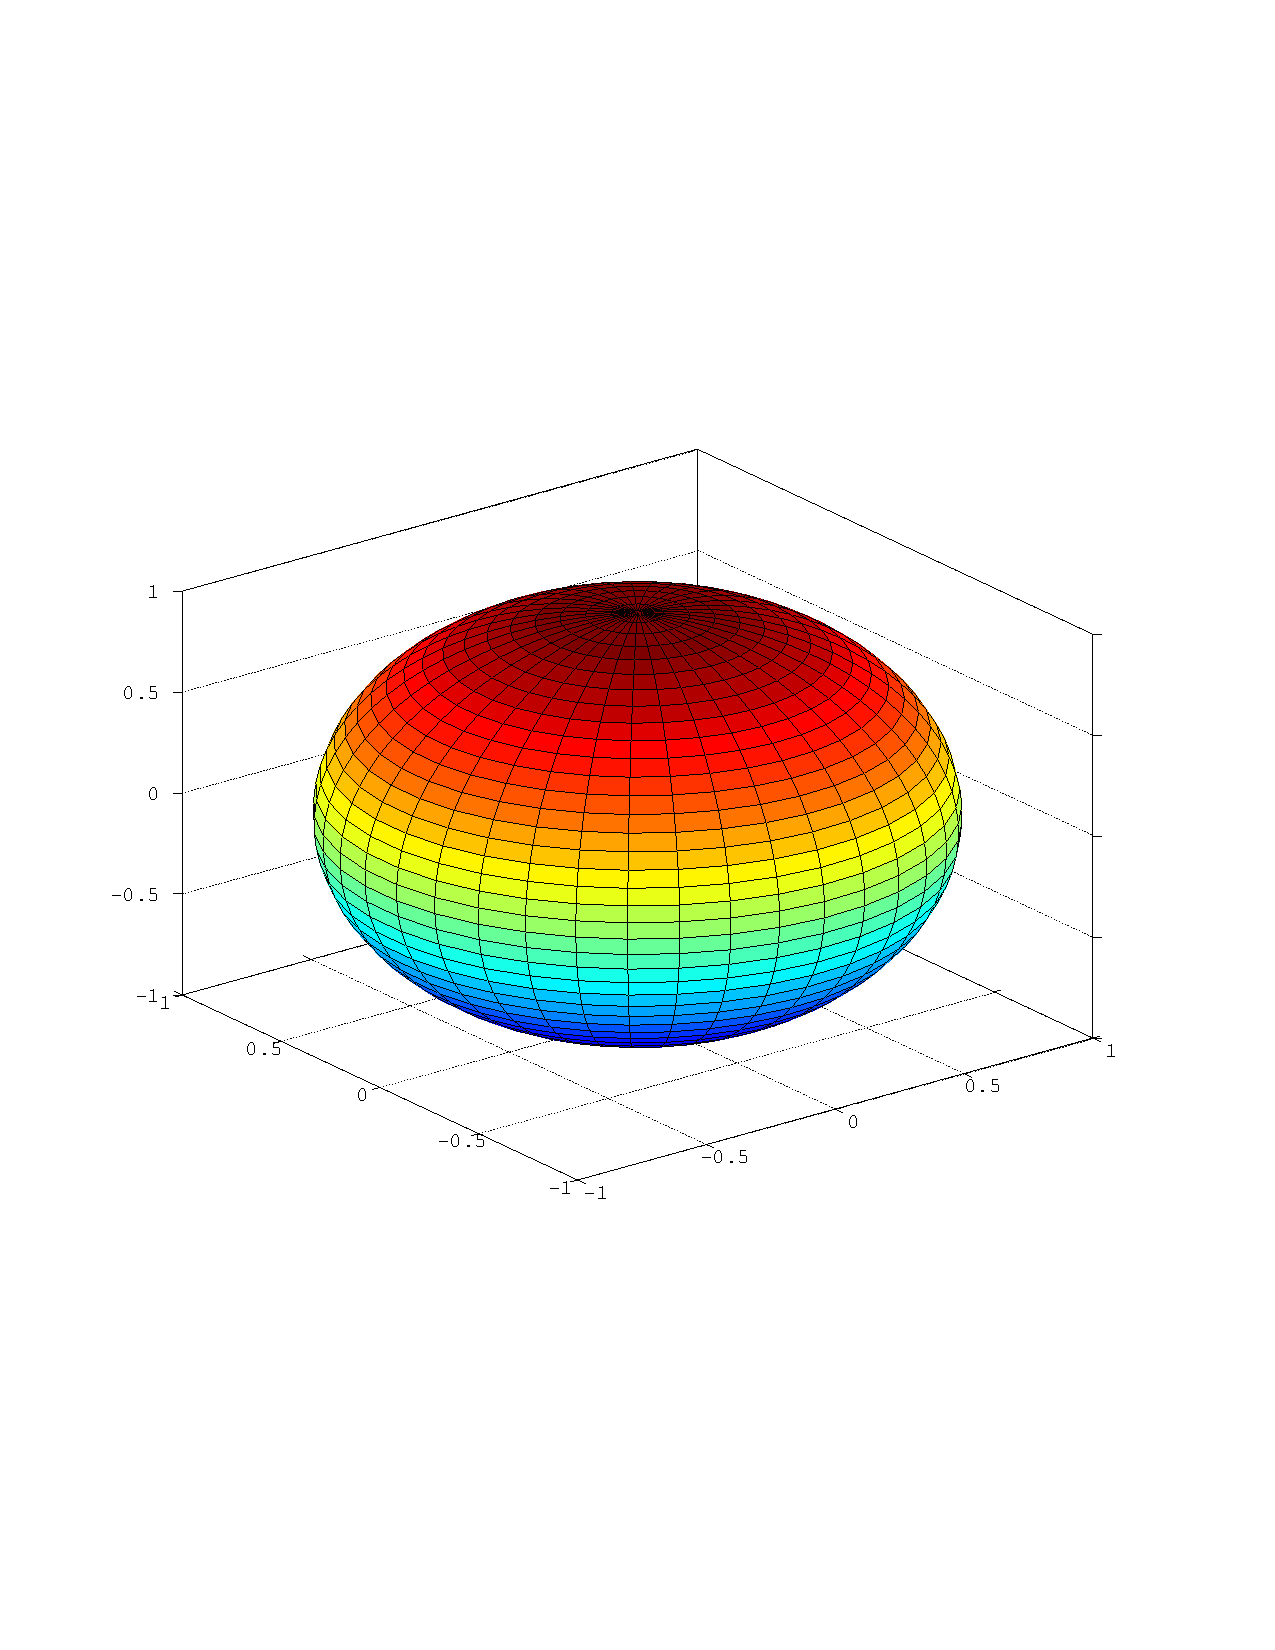
\includegraphics[scale=0.7]{elipsoide.pdf}
\end{figure}

\begin{figure}[!h]
	\centering
	\caption{Contornos do elips\'oide $\dfrac{x^2}{a^2} + \dfrac{y^2}{b^2} + \dfrac{z^2}{c^2} = 1$ pelo plano $z = k$}
	\hspace*{-2cm}
	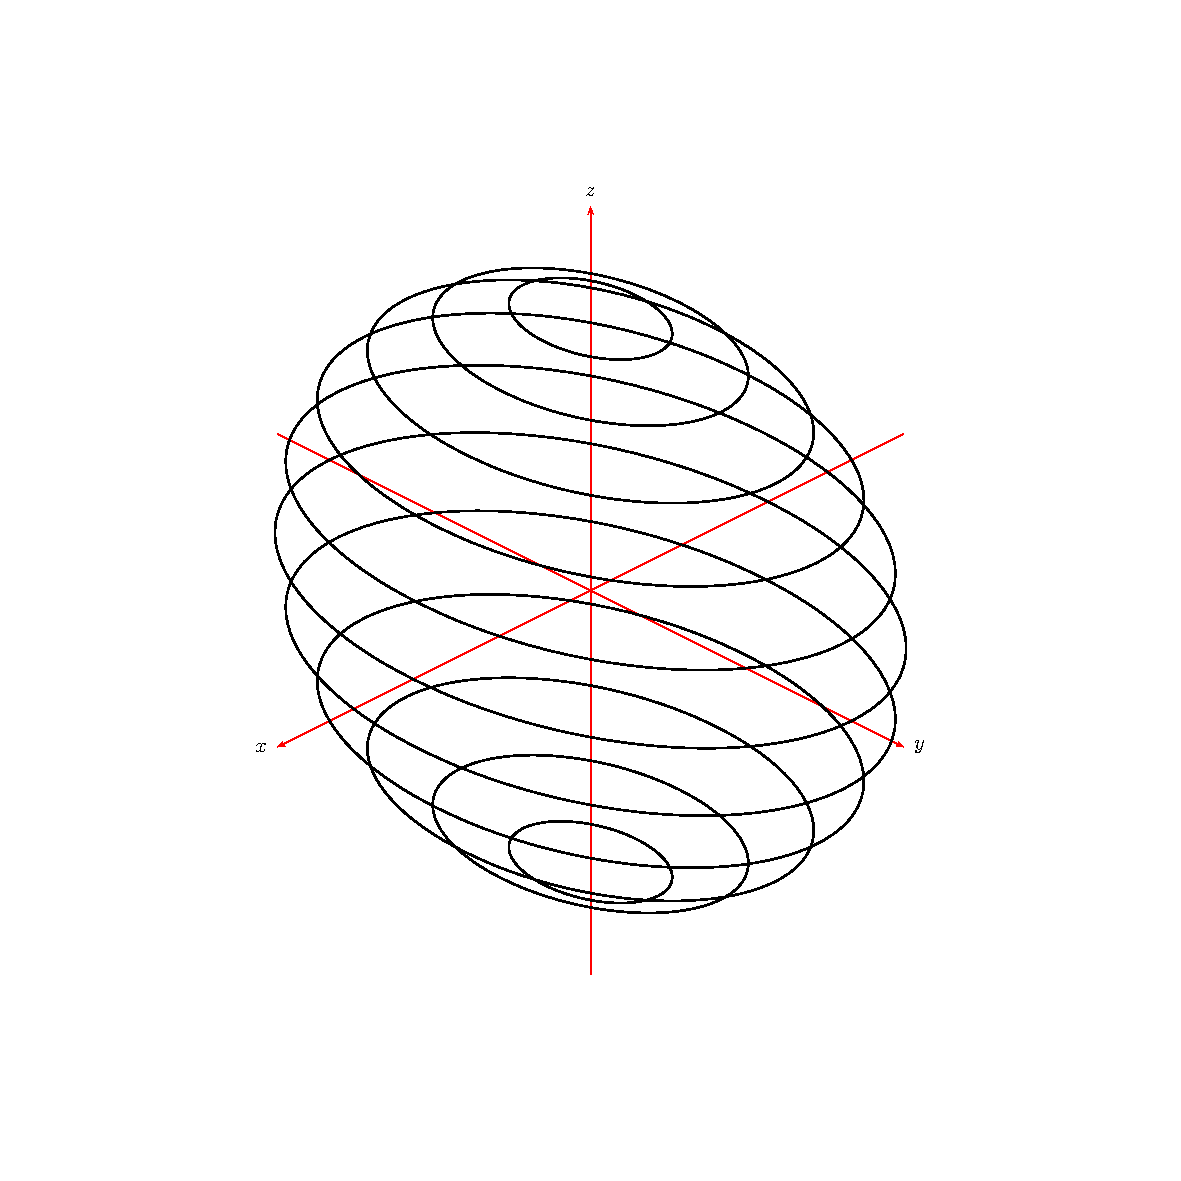
\includegraphics{elipsoide-contornos-eixo-z.pdf}
\end{figure}

% section elipsoide (end)

\section{Parabol\'oides} % (fold)
\label{sec:paraboloide}
\begin{definicao}
	Sejam $a$ e $b$ n\'umeros reais positivos a qu\'adrica descrita de equa\c{c}\~ao
	\[
		z = \dfrac{x^2}{a^2} + \dfrac{y^2}{b^2},
	\]
	\'e chamada de:
	\begin{enumerate}
		\item um \textbf{parabol\'oide el{\'\i}ptico} se $a \ne b$;\index{Qu\'adricas!Parabol\'oide el{\'\i}ptico}
		\item um \textbf{parabol\'oide de rota\c{c}\~ao} se $a = b$;\index{Qu\'adricas!Parabol\'oide de rota\c{c}\~ao}
	\end{enumerate}
\end{definicao}

A interse\c{c}\~ao do parabol\'oide
\[
	z = \dfrac{x^2}{a^2} + \dfrac{y^2}{b^2},
\]
com o plano $\pi: x = k$ \'e dada por
\[
	z = \dfrac{k^2}{a^2} + \dfrac{y^2}{b^2},
\]
que \'e uma par\'abola. O mesmo ocorrer\'a com o plano $\pi: y = k$.

Agora a interse\c{c}\~ao com $z = k$ \'e dada forma
\[
	\dfrac{x^2}{a^2} + \dfrac{y^2}{b^2} = k.
\]

Se $k < 0$, ent\~ao a interse\c{c}\~ao \'e vazia. Se $k = 0$, a interse\c{c}\~ao \'e o ponto $(0,0,0)$. Se $k > 0$, precisamos analisar o que ocorre com $a$ e $b$: se $a \ne b$, ent\~ao obtemos uma elipse. Se $a = b$, ent\~ao a interse\c{c}\~ao \'e uma circunfer\^encia.

\begin{definicao}
	Sejam $a$ e $b$ n\'umeros reais positivos. A qu\'adrica descrita pela equa\c{c}\~ao
	\[
		z = \dfrac{y^2}{b^2} - \dfrac{x^2}{a^2},
	\]
	\'e chamada de um um \textbf{parabol\'oide hiperb\'olico}.\index{Qu\'adricas!Parabol\'oide hiperb\'olico}
\end{definicao}

A interse\c{c}\~ao do parabol\'oide hiperb\'olico com o plano $\pi : z = k$ \'e dada por
\[
	\begin{cases}
		\dfrac{y^2}{b^2} - \dfrac{x^2}{a^2} = k\\
		z = k
	\end{cases}.
\]

Se $k = 0$, ent\~ao obtemos
\[
	\dfrac{y^2}{b^2} - \dfrac{x^2}{a^2} = \left(\dfrac{y}{b} - \dfrac{x}{a}\right)\left(\dfrac{y}{b} + \dfrac{x}{a}\right) = 0
\]
que trata-se de duas retas concorrentes na origem:
\[
	r : \begin{cases}
		\dfrac{y}{b} - \dfrac{x}{a} = 0\\
		z = 0
	\end{cases}, \quad s : \begin{cases}
		\dfrac{y}{b} - \dfrac{x}{a} = 0\\
		z = 0
	\end{cases}.
\]

Se $k \ne 0$, podemos escrever
\[
	\dfrac{y^2}{kb^2} - \dfrac{x^2}{ka^2} = 1
\]
que \'e uma hip\'erbole.

A interse\c{c}\~ao com o plano $\pi : y = k$ \'e dada por
\[
	z = \dfrac{k^2}{b^2} - \dfrac{x^2}{a^2}
\]
que \'e uma par\'abola. O mesmo ocorre com o plano $\pi : x = k$.


\begin{figure}[h]
	\centering
	\caption{Parabol\'oide El{\'\i}ptico: $z = \dfrac{x^2}{a^2} + \dfrac{y^2}{b^2}$}
	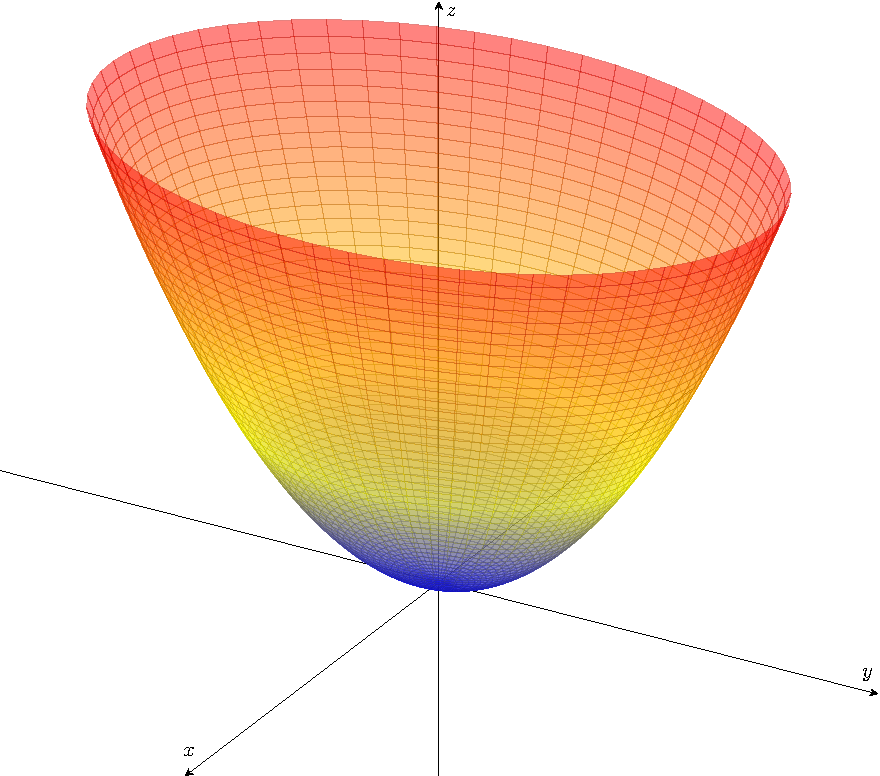
\includegraphics{paraboloide_eliptico.pdf}
\end{figure}

\begin{figure}[h]
	\centering
	\caption{Parabol\'oide Hiperb\'olico: $z = \dfrac{y^2}{b^2} - \dfrac{x^2}{a^2}$}
	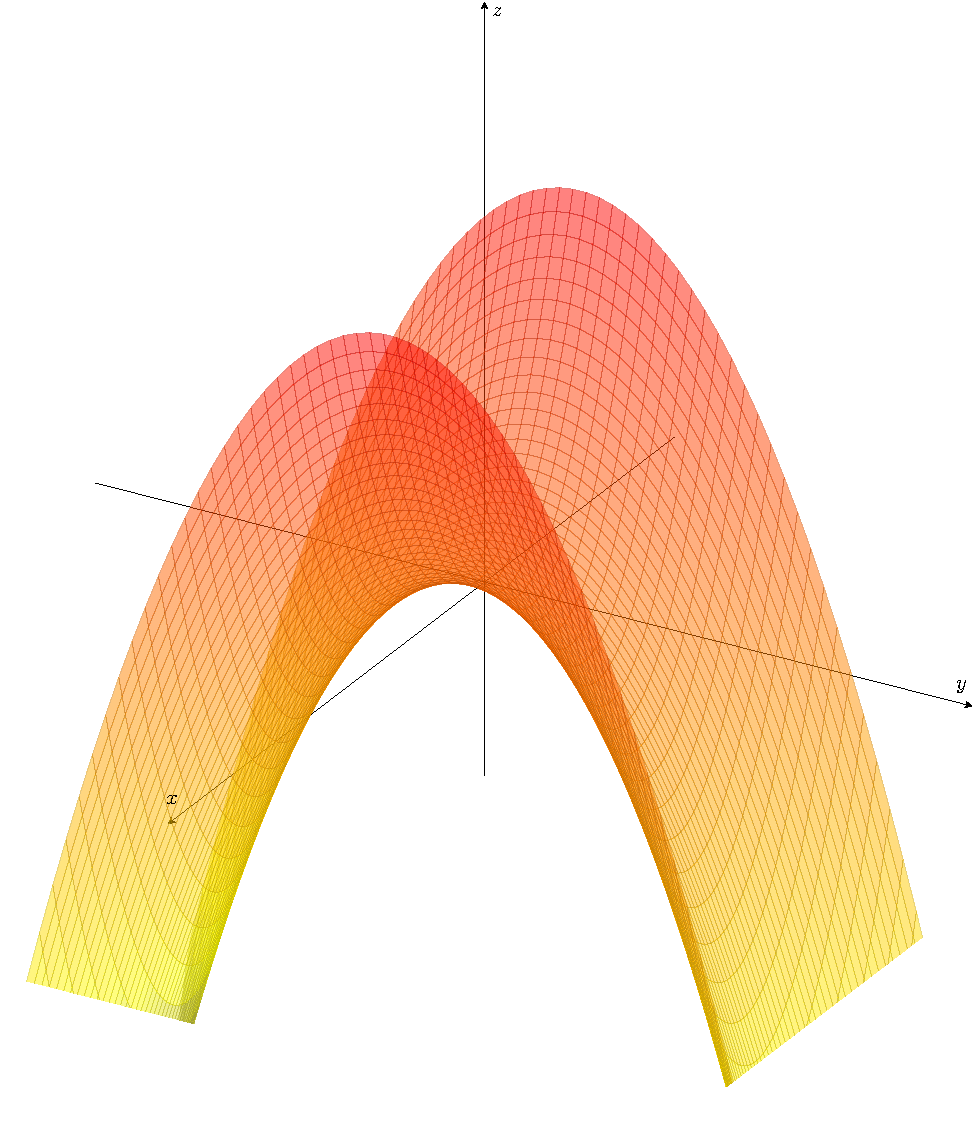
\includegraphics{paraboloide_hiperbolico.pdf}
\end{figure}
% section paraboloide (end)

\section{Hiperbol\'oides} % (fold)
\label{sec:hiperboloide}
\begin{definicao}
	Um \textbf{hiperbol\'oide de uma folha} \'e uma qu\'adrica descrita pela equa\c{c}\~ao
	\[
		\dfrac{x^2}{a^2} + \dfrac{y^2}{b^2} - \dfrac{z^2}{c^2} = 1
	\]
	onde os n\'umeros reais $a$, $b$ e $c$ s\~ao positivos e pelo menos dois deles s\~ao distintos.\index{Qu\'adricas!Hiperbol\'oide de uma folha}
\end{definicao}

Para o caso do hiperbol\'oide de uma folha a interse\c{c}\~ao com o plano $\pi : z = k$ \'e dada pelo sistema
\[
	\begin{cases}
		\dfrac{x^2}{a^2} + \dfrac{y^2}{b^2} = 1 + \dfrac{k^2}{c^2}\\
		z = k.
	\end{cases}
\]

Denotando $p = 1 + k^2/c^2 > 0$ podemos escrever
\begin{equation}\label{resultado_intersecao_hiperboloide_1_folha_planoz}
	\dfrac{x^2}{pa^2} + \dfrac{y^2}{pb^2} = 1.
\end{equation}

Se $a = b$, ent\~ao a equa\c{c}\~ao \eqref{resultado_intersecao_hiperboloide_1_folha_planoz} descreve uma circunfer\^encia. Se $a \ne b$, ent\~ao a equa\c{c}\~ao \eqref{resultado_intersecao_hiperboloide_1_folha_planoz} descreve uma elipse.

Agora a interser\c{c}\~ao com o plano $\pi : y = k$ \'e descrita pela equa\c{c}\~ao
\begin{equation}\label{intersecao_hiperboloide_1_folha_planoy}
	\dfrac{x^2}{a^2} - \dfrac{z^2}{c^2} = 1 - \dfrac{k^2}{b^2}.
\end{equation}
Se $k^2 = b^2$, obtemos
\[
	\dfrac{x^2}{a^2} - \dfrac{z^2}{c^2} = 0,	
\]
isto \'e,
\[
	\left(\dfrac{x}{a} - \dfrac{z}{c}\right)\left(\dfrac{x}{a} + \dfrac{z}{c}\right).
\]
Logo a interse\c{c}\~ao de $\pi$ com o hiperbol\'oide de uma folha \'e o par de retas concorrentes
\[
	r : \begin{cases}
		\dfrac{x}{a} - \dfrac{z}{c} = 0\\
		y = k
	\end{cases}, \quad s : \begin{cases}
		\dfrac{x}{a} + \dfrac{z}{c} = 0\\
		y = k
	\end{cases}.
\]

Se $k^2 \ne b^2$, ent\~ao fazendo $p = 1 - k^2/b^2$ podemos escrever a equa\c{c}\~ao \eqref{intersecao_hiperboloide_1_folha_planoy} como
\[
	\dfrac{x^2}{pa^2} - \dfrac{z^2}{pc^2} = 1	
\]
obtendo-se uma hip\'erbole.

De modo an\'alogo, obtemos as mesmas interse\c{c}\~oes se considerarmos o plano $\pi : x = k$.
\begin{figure}[h]
	\centering
	\caption{Hiperbol\'oide de uma folha: $\dfrac{x^2}{a^2} + \dfrac{y^2}{b^2} - \dfrac{z^2}{c^2} = 1$}
	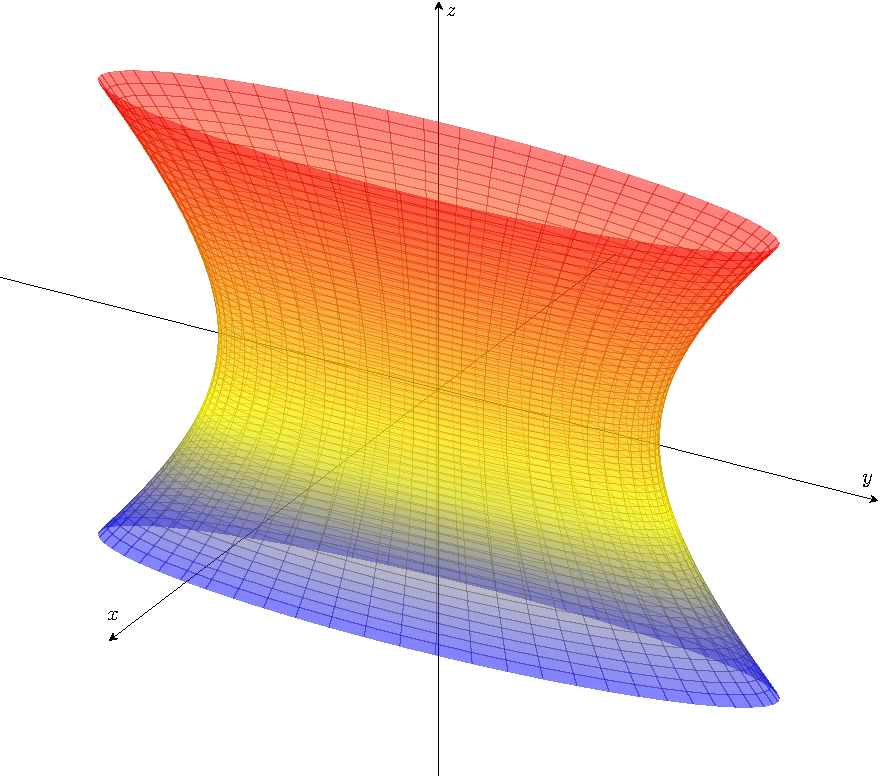
\includegraphics{hiperboloide_uma_folha.pdf}
\end{figure}

\begin{definicao}
	Um \textbf{hiperbol\'oide de duas folhas} \'e uma qu\'adrica descrita pela equa\c{c}\~ao
	\[
		\dfrac{y^2}{b^2} - \dfrac{x^2}{a^2} - \dfrac{z^2}{c^2} = 1
	\]
	onde os n\'umeros reais $a$, $b$ e $c$ s\~ao positivos e pelo menos dois deles s\~ao distintos.\index{Qu\'adricas!Hiperbol\'oide de duas folhas}
\end{definicao}

A interse\c{c}\~ao do hiperbol\'oide de duas folhas com a plano $\pi: z = k$ \'e dada por
\[
	\dfrac{y^2}{b^2} - \dfrac{x^2}{a^2} = 1 +  \dfrac{k^2}{c^2}.
\]
Denotando $p = 1 + k^2/c^2$ podemos escreve a equa\c{c}\~ao anterior como
\[
	\dfrac{y^2}{pb^2} - \dfrac{x^2}{pa^2} = 1
\]
que representa uma hip\'erbole.

A interse\c{c}\~ao com o plano $\pi: x = k$ \'e dada por
\[
	\dfrac{y^2}{b^2} - \dfrac{z^2}{c^2} = 1 +  \dfrac{k^2}{b^2}.
\]
e fazendo $p = 1 + k^2/b^2$ obtemos
\[
	\dfrac{y^2}{pb^2} - \dfrac{z^2}{pc^2} = 1
\]
que tamb\'em \'e uma hip\'erbole.

Agora a interse\c{c}\~ao com o plano $\pi : y = k$ \'e dada por
\begin{equation}\label{intersecao_hiperboloide_2_folhas_planoy}
	\dfrac{x^2}{a^2} + \dfrac{z^2}{c^2} = \dfrac{k^2}{c^2} - 1.	
\end{equation}

Se $k^2 < b^2$, ent\~ao $k^2/b^2 - 1 < 0$ e da{\'\i} a equa\c{c}\~ao \eqref{intersecao_hiperboloide_2_folhas_planoy} n\~ao admite solu\c{c}\~ao.

Se $k^2 = k^2$, ent\~ao a interse\c{c}\~ao \'e ou o ponto $(0,k,0)$ ou o ponto $(0,-k,0)$.

Se $k^2 > b^2$, isto \'e, $k < -b$ ou $k > b$, ent\~ao tomando $p = k^2/b^2 - 1 > 0$, podemos escrever \eqref{intersecao_hiperboloide_2_folhas_planoy} como
\[
	\dfrac{x^2}{pa^2} + \dfrac{z^2}{pc^2} = 1.
\]
Assim se $a = c$, ent\~ao obtemos uma circunfer\^encia e se $a \ne c$, ent\~ao a interse\c{c}\~ao \'e uma elipse.

\begin{figure}[h]
	\centering
	\caption{Hiperbol\'oide duas folhas: $-\dfrac{x^2}{a^2} - \dfrac{y^2}{b^2} + \dfrac{z^2}{c^2} = 1$}
	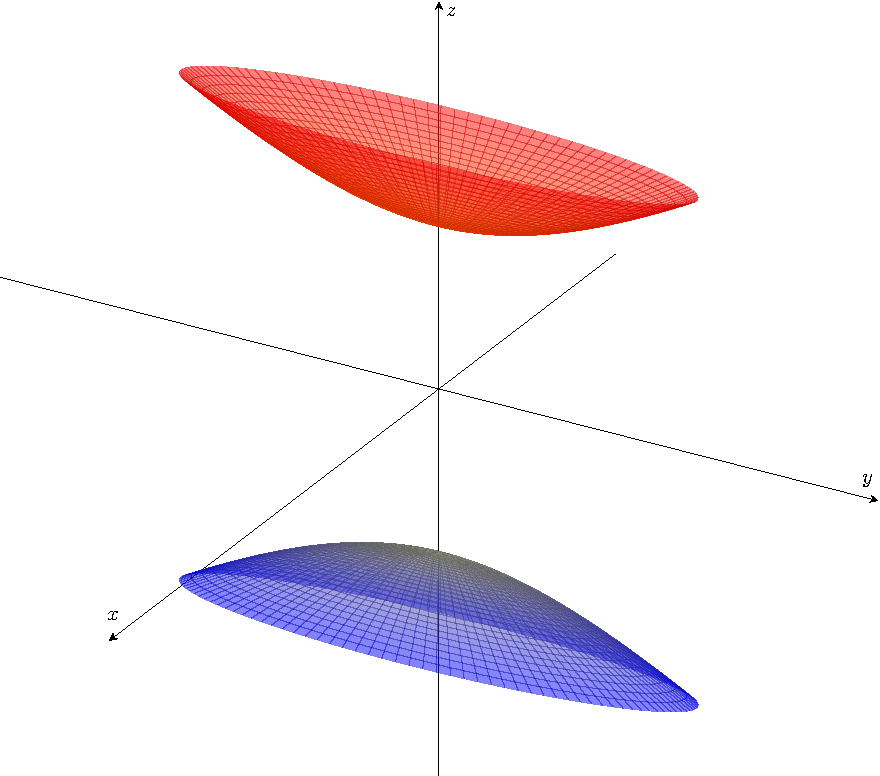
\includegraphics{hiperboloide_duas_folhas.pdf}
\end{figure}

% section hiperboloide (end)


% \begin{figure}
	


% 	\parametricplotThreeD[plotstyle=curve,yPlotpoints=20](0,360)(0,1){t cos 2 mul u mul t sin u mul u dup mul 2 add}
% \end{figure}

\section{Identifica\c{c}\~ao de Qu\'adricas} % (fold)
\label{sec:identificacao_de_quadricas}

Considere uma qu\'adrica de equa\c{c}\~ao
\begin{equation}\label{equacao_geral_quadrica}
  ax^2 + by^2 + cz^2 + dxy + exz + fyz + gx + hy + iz + j = 0.
\end{equation}

Queremos remover os termos $xy$, $xz$ e $yz$ da equa\c{c}\~ao \eqref{equacao_geral_quadrica} para ent\~ao usar uma transla\c{c}\~ao de eixos, se necess\'ario, e com isso identicar a c\^onica definida por tal equa\c{c}\~ao. Para isso vamos tentar encontrar uma matriz $Q = [\vec{U_1}\ \vec{U_2}\ \vec{U_3}]$ onde os vetores $\vec{U_1}$, $\vec{U_2}$ e $\vec{U_3}$ s\~ao unit\'arios, ortogonais e tais que a mudan\c{c}a
\begin{equation}\label{substituicao_quadrica}
	\begin{bmatrix}
		x\\
		y\\
		z
	\end{bmatrix} = Q \begin{bmatrix}
		x_1\\
		y_1\\
		z_1
	\end{bmatrix}
\end{equation}
transforma a equa\c{c}\~ao \eqref{equacao_geral_quadrica} numa equa\c{c}\~ao da forma
\begin{equation}\label{equacao_rotacionada_quadrica}
  a'x_1^2 + b'y_1^2 c'z_1^2 + g'x_1 + h'y_1 i'z + j = 0.
\end{equation}

Inicialmente observe que a \eqref{equacao_geral_quadrica} pode ser escrita na forma
\begin{equation}\label{equacao_matricial_quadrica}
  X^tAX + KX + F = [0]
\end{equation}
onde
\[
  A = \begin{bmatrix}
    a & d/2 & e/2\\
    d/2 & b & f/2\\
    e/2 & f/2 & c
  \end{bmatrix}
, \quad K = \begin{bmatrix}
  g & h & i
\end{bmatrix}, \quad X = \begin{bmatrix}
  x\\
  y\\
  z
\end{bmatrix}\quad\mbox{e}\quad J = [j]
\]
e $t$ denota a matriz transposta. Queremos fazer uma substitui\c{c}\~ao da forma \eqref{substituicao_quadrica}, isto \'e, $X = QX'$ para com isso obter uma equa\c{c}\~ao na forma
\[
	X_1^tBX_1 + K'X_1 + J = 0
\]
onde
\[
	B = \begin{bmatrix}
		a' & d'/2 & e'/2\\
		d'/2 & b' & f'/2\\
		e'/2 & f'/2 & c'
	\end{bmatrix} = Q^tAQ,\quad K' = \begin{bmatrix}
		g' & h' & i'
	\end{bmatrix} = KQ,\quad X = \begin{bmatrix}
		x\\y\\z
	\end{bmatrix},\quad X_1 = \begin{bmatrix}
		x_1\\y_1\\z_1
	\end{bmatrix}.
\]

Agora observe que a matriz $Q$ \'e formada por vetores unit\'arios e ortogonais, da{\'\i} $Q^tQ = I_3$ e com isso obtemos
\begin{align*}
  B - \lambda I_3 = Q^t A Q - \lambda I_3 = Q^t A Q - Q^t (Q I_3) Q = Q^t (A - \lambda I_3)Q
\end{align*}
para todo $\lambda \in \real$. Com isso
\begin{align*}
  \det(B - \lambda I_3) = \det[Q^t(A - \lambda I_3)Q] = \det(Q^t)\det(A - \lambda I_3)\det(Q) = \det(A - \lambda I_3).
\end{align*}

Assim escolhendo a matriz $Q$ de tal forma que $d' = e' = f' = 0$, o que \'e sempre poss{\'\i}vel, obtemos
\begin{align*}
  \det(A - \lambda I_3) = \det(B - \lambda I_3) = \det \begin{bmatrix}
    a' - \lambda & 0 & 0\\
    0 & b' - \lambda & 0\\
    0 & 0 & c' - \lambda
  \end{bmatrix} = -(\lambda - a')(\lambda - b')(\lambda - c').
\end{align*}

Logo os coeficientes $a'$, $b'$ e $c'$ s\~ao ra{\'\i}zes da equa\c{c}\~ao de terceiro grau
\begin{equation}
  p(\lambda) = \det(A - \lambda I_3) = \det \begin{bmatrix}
    a - \lambda & d/2 & e/2\\
    d/2 & b - \lambda & f/2\\
    e/2 & f/2 & c - \lambda
  \end{bmatrix}.
\end{equation}

Agora para determinar a matriz $Q$ come\c{c}amos com a equa\c{c}\~ao
\[
  B = Q^t A Q
\]
e multiplicamos \`a esquerda por $Q$ obtendo
\[
  Q B = AQ.
\]
Mas
\[
	AQ = A \begin{bmatrix}
		\vec{U_1} & \vec{U_2} e \vec{U_3}
	\end{bmatrix} = \begin{bmatrix}
		A\vec{U_1} & A\vec{U_2} e A\vec{U_3}
	\end{bmatrix}
\]
e
\[
	QB = \begin{bmatrix}
		\vec{U_1} & \vec{U_2} e \vec{U_3}
	\end{bmatrix}\begin{bmatrix}
		a' & 0 & 0\\
		0 & b' & 0\\
		0 & 0 & c'
	\end{bmatrix} = \begin{bmatrix}
		a'\vec{U_1} & b'\vec{U_2} e c'\vec{U_3}
	\end{bmatrix}.
\]
Da{\'\i} $\vec{U_1}$, $\vec{U_2}$ e $\vec{U_3}$ devem satisfazer as equa\c{c}\~oes
\[
	A\vec{U_1} = a'\vec{U_1},\quad A\vec{U_2} = b'\vec{U_2} \quad A\vec{U_3} = c'\vec{U_3}.
\]

Da primeira equa\c{c}\~ao obtemos
\begin{align*}
	A\vec{U_1} = a'I_3\vec{U_1}\\
	(A - a'I_3)\vec{U_1} = \vec{0}.
\end{align*}

Logo $\vec{U_1}$ \'e uma solu\c{c}\~ao de norma 1 do sistema linear
\[
  (A - a'I_3)X = [0].
\]
Analogamente, $\vec{U_2}$ \'e uma solu\c{c}\~ao de norma 1 do sistema linear
\[
  (A - b'I_3)X = [0],
\]
que seja ortogonal a $\vec{U_1}$. O terceiro vetor $\vec{U_3}$ \'e obtido de forma an\'aloga e deve ser ortogonal tanto a $\vec{U_1}$ quanto a $\vec{U_2}$, assim podemos tomar
\[
	\vec{U_3} = \vec{U_1}\times\vec{U_2}.
\]
Como $\vec{U_1}$ e $\vec{U_2}$ s\~ao de norma 1, ent\~ao $\vec{U_3}$ tamb\'em \'e de norma 1.

Portanto a mudan\c{c}a que elemina os termos $xy$, $xz$ e $yz$ \'e dada por $Q = [\vec{U_1}\ \vec{U_2}\ \vec{U_3}]$. Assim temos o seguinte teorema:

\begin{teorema}
  Considere a equa\c{c}\~ao
  \[
      ax^2 + by^2 + cz^2 + dxy + exz + fyz + gx + hy + iz + j = 0
  \]
  com $a$, $b$, $c$, $d$, $e$, $f$, $g$, $h$, $i$, $j \in \real$, sendo $a$, $b$, $c$, $d$, $e$ e $f$ n\~ao necessariamente nulos. Ent\~ao mediante uma mudan\c{c}a da forma
  \[
    X = Q X_1
  \]
  onde
  \[
    X = \begin{bmatrix}
      x\\y\\z
    \end{bmatrix}, \quad
    Q = \begin{bmatrix}
    	\vec{U_1} & \vec{U_2} & \vec{U_3}
  \end{bmatrix}, \quad\mbox{e}\quad
  X_1 = \begin{bmatrix}
    x_1\\y_1\\z_1
  \end{bmatrix}
  \]
  a equa\c{c}\~ao da geral da qu\'adrica acima pode ser transformada em
  \[
    a'x_1^2 + b'y_1^2 + c'z_1^2 + g'x_1 + h'y_1 + i'z_1 + j = 0
  \]
  em que $a'$, $b'$ e $c'$ s\~ao ra{\'\i}zes de
  \[
    p(\lambda) = \det(A - \lambda I_3) = \det \begin{bmatrix}
      a - \lambda & d/2 & e/2\\
      d/2 & b - \lambda & f/2\\
      e/2 & f/2 & c - \lambda
    \end{bmatrix}.
  \]

  Mais ainda, $\vec{U_1}$ \'e uma solu\c{c}\~ao de norma 1 do sistema linear
  \[
    \begin{bmatrix}
      a - a' & d/2 & e/2\\
      d/2 & b - a' & f/2\\
      e/2 & f/2 & c - a'
    \end{bmatrix} \begin{bmatrix}
      x\\y\\z
    \end{bmatrix} = \begin{bmatrix}
      0\\0\\z
    \end{bmatrix},
  \]
  $\vec{U_2}$ \'e uma solu\c{c}\~ao de norma 1 do sistema linear
  \[
    \begin{bmatrix}
      a - b' & d/2 & e/2\\
      d/2 & b - b' & f/2\\
      e/2 & f/2 & c - b'
    \end{bmatrix} \begin{bmatrix}
      x\\y\\z
    \end{bmatrix} = \begin{bmatrix}
      0\\0\\z
    \end{bmatrix},
  \]
  e
  \[
  	\vec{U_3} = \vec{U_1} \times \vec{U_2}
  \]
\end{teorema}

\begin{teorema}
  Seja $\mathcal{S}$ o conjunto dos pontos do espa\c{c}o que satisfazem a equa\c{c}\~ao
  \[
    ax^2 + by^2 + cz^2 + dxy + exz + fyz + gx + hy + iz + j = 0,
  \]
  com $a$, $b$, $c$, $d$, $e$, $f$, $g$, $h$, $i$, $j \in \real$, sendo $a$, $b$, $c$, $d$, $e$ e $f$ n\~ao simultaneamente nulos. Sejam $a'$, $b'$ e $c'$ ra{\'\i}zes de
  \[
    p(\lambda) = \det \begin{bmatrix}
      a - \lambda & d/2 & e/2 \\
      d/2 & b - \lambda & f/2\\
      e/2 & f/2 & c - \lambda
    \end{bmatrix}.
  \]
  \begin{enumerate}[label=({\roman*})]
    \item Se $a'$, $b'$ e $c'$ tiverem o mesmo sinal, ent\~ao $\mathcal{S}$ \'e um elips\'oide, um ponto ou o conjunto vazio.
    \item Se $a'$, $b'$ e $c'$ forem n\~ao nulos e n\~ao tiverem o mesmo sinal, ent\~ao $\mathcal{S}$ \'e um hip\'erbol\'oide de uma folha, de duas folhas ou um cone el{\'\i}ptico.
    \item Se apenas um entre $a'$, $b'$ e $c'$ for nulo, ent\~ao $\mathcal{S}$ \'e um par\'abol\'oide el{\'\i}ptico, hiperb\'olico, um cil{\'\i}ndro el{\'\i}ptico, hiperb\'olico, dois planos concorrentes, uma reta ou o conjunto vazio.
    \item Se exatamente dois entre $a'$, $b'$ e $c'$ forem nulos, ent\~ao $\mathcal{S}$ \'e um cilindro parab\'olico, um par de planos paralelos ou um plano.
  \end{enumerate}
\end{teorema}



% section identificacao_de_quadricas (end)


% chapter quadricas (end)